\documentclass[twoside,twocolumn]{article}

\usepackage{blindtext} % Package to generate dummy text throughout this template 

\usepackage[sc]{mathpazo} % Use the Palatino font
\usepackage[T1]{fontenc} % Use 8-bit encoding that has 256 glyphs
\linespread{1.05} % Line spacing - Palatino needs more space between lines
\usepackage{microtype} % Slightly tweak font spacing for aesthetics

\usepackage[english]{babel} % Language hyphenation and typographical rules

\usepackage[hmarginratio=1:1,top=32mm, left=15truemm, right=15truemm, columnsep=20pt]{geometry} % Document margins
\usepackage[hang, small,labelfont=bf,up,textfont=it,up]{caption} % Custom captions under/above floats in tables or figures
\usepackage{booktabs} % Horizontal rules in tables

\usepackage{lettrine} % The lettrine is the first enlarged letter at the beginning of the text

\usepackage{enumitem} % Customized lists
\setlist[itemize]{noitemsep} % Make itemize lists more compact

\usepackage{abstract} % Allows abstract customization
\renewcommand{\abstractnamefont}{\normalfont\bfseries} % Set the "Abstract" text to bold
\renewcommand{\abstracttextfont}{\normalfont\small\itshape} % Set the abstract itself to small italic text

\usepackage{titlesec} % Allows customization of titles
\usepackage{graphicx}
\renewcommand\thesection{\Roman{section}} % Roman numerals for the sections
\renewcommand\thesubsection{\roman{subsection}} % roman numerals for subsections
\titleformat{\section}[block]{\large\scshape\centering}{\thesection.}{1em}{} % Change the look of the section titles
\titleformat{\subsection}[block]{\large}{\thesubsection.}{1em}{} % Change the look of the section titles

\usepackage{fancyhdr} % Headers and footers
\pagestyle{fancy} % All pages have headers and footers
\fancyhead{} % Blank out the default header
\fancyfoot{} % Blank out the default footer
\fancyfoot[RO,LE]{\thepage} % Custom footer text

\usepackage{titling} % Customizing the title section

\usepackage{hyperref} % For hyperlinks in the PDF
\usepackage{algorithm, algorithmic}
\usepackage{amsmath}
\usepackage{bm}
\renewcommand{\algorithmicrequire}{\textbf{Input:}}
\renewcommand{\algorithmicensure}{\textbf{Output:}}
\newcommand{\argmax}{\mathop{\rm arg~max}\limits}
\newcommand{\argmin}{\mathop{\rm arg~min}\limits}
\newcommand{\E}{\mathbb{E}}
%----------------------------------------------------------------------------------------
%	TITLE SECTION
%----------------------------------------------------------------------------------------

\setlength{\droptitle}{-4\baselineskip} % Move the title up

\pretitle{\begin{center}\Huge\bfseries} % Article title formatting
\posttitle{\end{center}} % Article title closing formatting
\title{Mixed Autonomy Reducing Congestion \newline with Reinforcement Learning} % Article title
\author{Toshinori Kitamura}
\date{\today} % Leave empty to omit a date
\renewcommand{\maketitlehookd}{%
\begin{abstract}
\noindent 

This research demonstrates the potential of multi-agent reinforcement learning to reduce traffic congestion. The main goal is to solve the remaining problems of \cite{Kreidieh2018}, which uses only a single agent to control all the RL cars on the road. If we use a single agent, the number of the cars is not flexible, and it is not safe from the view of cyber security. Instead, this research focus on multi-agent method and solve the problems by modifying state space and reward function. Since the reward design is difficult for this task, an imitation learning algorithm GAIL is applied to the traffic control as another experiment.
\end{abstract}
}

%----------------------------------------------------------------------------------------

\begin{document}
\setlength{\abovedisplayskip}{0.5pt}
\setlength{\belowdisplayskip}{0.5pt}

\maketitle
\section{Introduction\label{introduction}}

This paper shows an application of reinforcement learning for congestion reduction by mixed-autonomy, where both automated and human-driven vehicles present on traffic\cite{Wu:EECS-2018-132}. Some studies demonstrate that even a small number of vehicles in congested traffic can reduce huge amount of fuel consumption\cite{Wu:EECS-2018-132}.\\
Since 28\% of energy consumption in the U.S. is due to the transportation\cite{U.S.EnergyInformationAdministration2017}, and congestion can increase the fuel consumption\cite{Treiber2008}, reducing traffic congestion saves large amount of energy. 
To control the system-level traffic velocity, both model-based and model-free methods have been studied so far. The model-based methods give analytical solutions to maximize the traffic efficiency, but the situation it can be utilized is very limited. For example, the model-based controllers "Follower Stopper" and "PI with Saturation" \cite{Stern2018} can reduce the congestion in a ring road, but it doesn't give the optimal solution in the complex environments such as bottleneck and figure-eight(see Fig.\ref{fig:envs}). Due to the complex model of the real world traffic, the model-based methods may not work in many situations. 

On the other hand, model-free reinforcement learning(RL) has a potential to solve complex problems. For example, \cite{Mnih2013} trains an agents which solves Atari games at superhuman levels, and \cite{Silver2017} demonstrates that a RL agent outperforms a human Go player. \cite{Vinitsky2018} applies some state-of-the-art RL algorithms to complex traffic shown in Fig. \ref{fig:envs}, and most of the methods achieve better score than the situation with only human driven car. 

This research extends that previous work\cite{Kreidieh2018} and develops more practical agent using multi-agents method. A remaining problem in \cite{Kreidieh2018} is that it only uses one agent to control multiple cars. It's not flexible when the number of the car changes. Moreover, from the view of cyber security, one master node controlling the acceleration of multiple cars is dangerous. To train the agents, a policy gradient algorithm, Proximal Policy Optimization(PPO)\cite{Schulman2017} is used. The traffic simulator used in this work is Flow\cite{Wu2017}. It contains some benchmarks of practical traffic situations shown as \ref{fig:envs}, and it is easy to apply reinforcement learning agents to Flow. 

Finally, this paper shows the performance of imitation learning for the traffic control task. Generally, it is difficult to design a reward function for reinforcement learning. One of the solutions for reward design problem is to learn from an expert agent using imitation learning. To apply imitation learning, Generative Adversarial Imitation Learning(GAIL)\cite{Ho} is used in this research.

\begin{figure}[]
    \begin{center}
    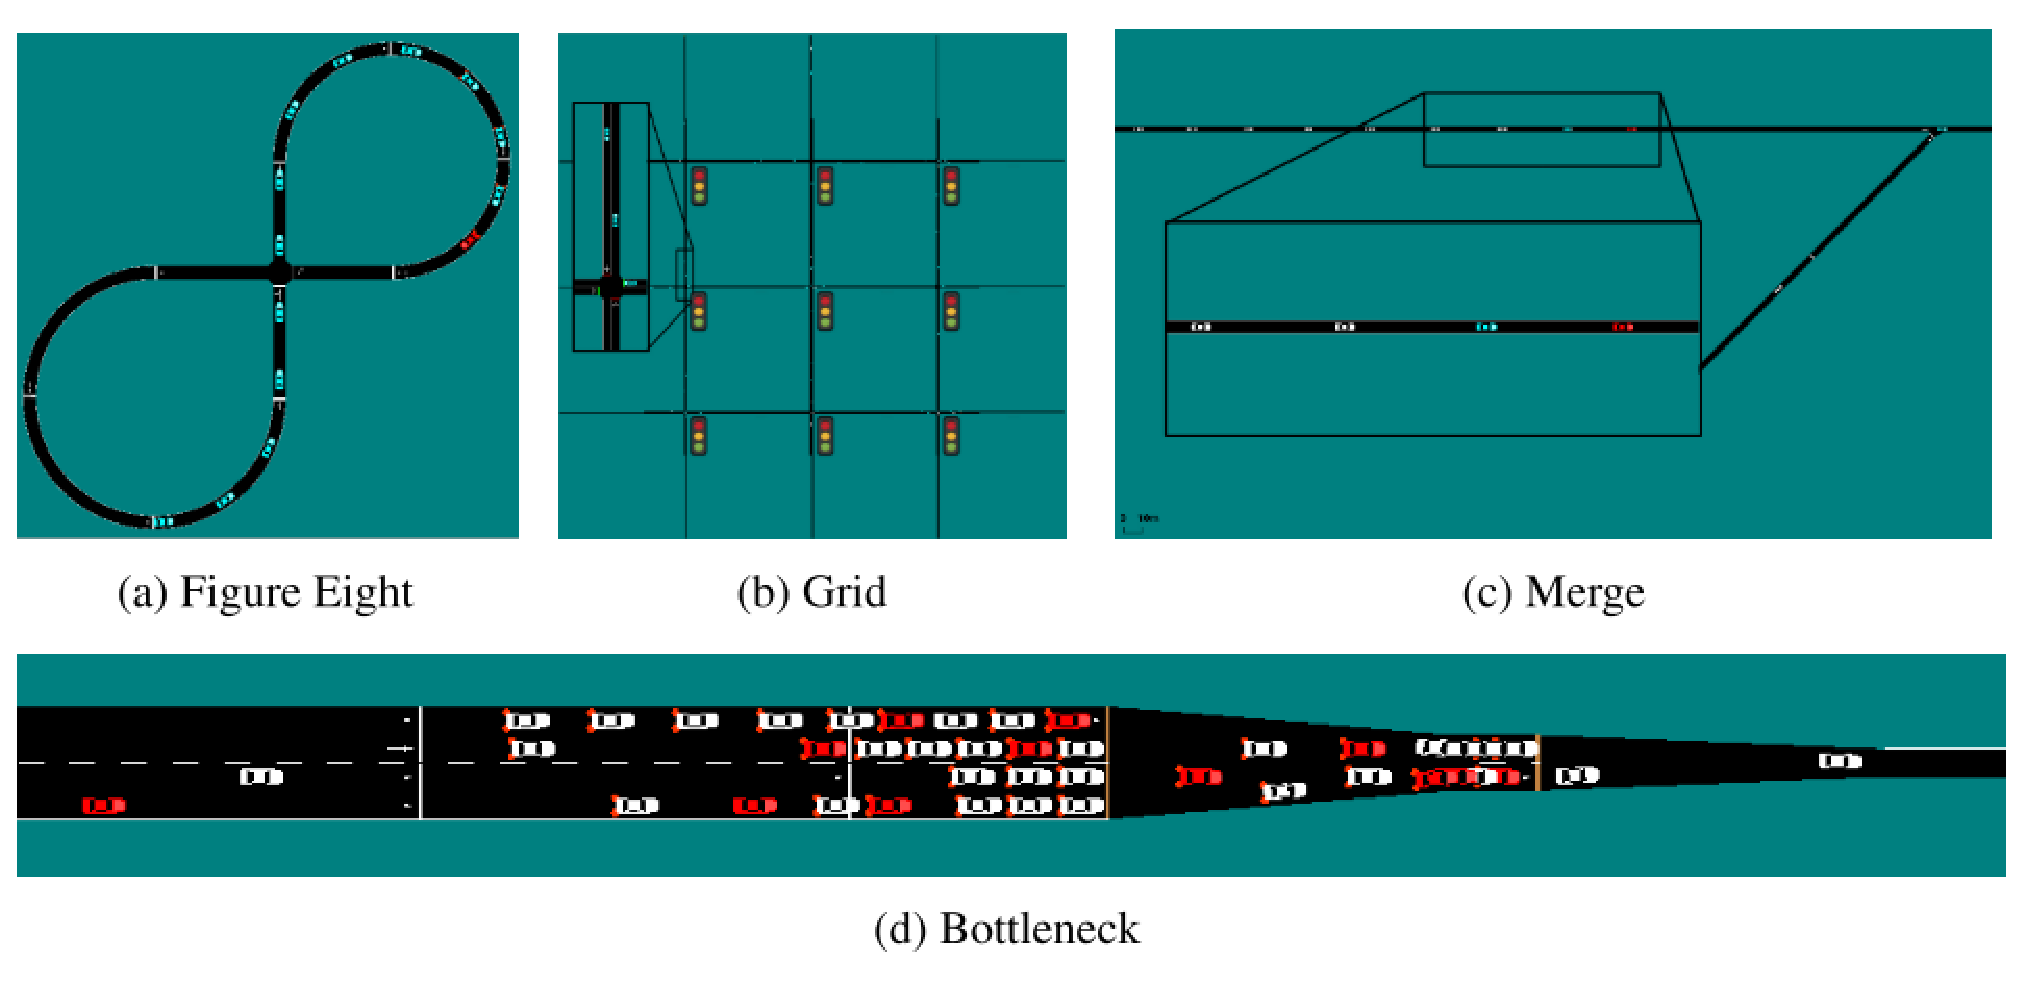
\includegraphics[width=9cm]{img/envs.eps}
    \caption{Complex traffic environments in "flow" (cited from \cite{Vinitsky2018})}
    \label{fig:envs}
    \end{center}
\end{figure}
%ここに画像が入る また、FLOWの結果を出して強化学習のほうが最適解を出せることを示す。
\section{Background\label{background}}

\subsection{Reinforcement Learning}

RL is an optimization algorithm in Markov decision process(MDP), defined by $\left(\mathcal{S}, \mathcal{A}, \mathcal{P}, r, \rho_{0}, \gamma, T\right)$. Here, $\mathcal{S}$ is a state space, $\mathcal{A}$ is an action space, $\mathcal{P}$ is a state transition probability function, $r$ is a reward function, $\rho_{0}$ is initial state distribution, $\gamma$ is a discount factor, and $T$ is a time horizon.

In RL algorithms, agents interact the environment and try to learn a parameterized policy $\pi_\theta$ which maximize the sum of the discounted reward $\sum_{i=0}^{T} \gamma^{i} r_{i}$, i.e. $\pi_\theta = \argmax_{\pi_\theta} \sum_{i=0}^{T} \gamma^{i} r_{i}$. The rewards are sampled from the trajectory $\tau=\left(s_{0}, a_{0}, \ldots, a_{T-1}, s_{T}\right)$. The initial states, actions and the next states are sampled as $s_{0} \sim \rho_{0}\left(s_{0}\right)$, $a_{t} \sim \pi_{\theta}\left(a_{t}\right)$, and $s_{t+1} \sim \mathcal{P}\left(s_{t+1} | s_{t}, a_{t}, a_{t}\right)$

The plain policy gradient(PG) method updates the parameter using following gradient.

\begin{equation} \label{eq:PG}
\nabla J\left(\pi_{\theta}\right)=E\left[\nabla_{\theta} \log \pi_{\theta}(a | s) Q_{\pi}(s, a)\right]
\end{equation}

$Q_{\pi}$ is an action value function. The problem of plain PG is its instability. Intuitively, the instability is from the term $\nabla_{\theta} \log \pi_{\theta}(a | s)$. As the training goes, the policy is getting deterministic, and the gradient of the policy becomes large around its mean value. PPO solves the problem by restricting the update in parameter space, and achieves stabler RL training.

\subsection{Imitation Learning}

Designing reward function is difficult problem in RL. Instead, IL trains the agents from the trajectory generated by an expert. \cite{Ho} shows that the IL problem is same as a problem finding a policy whose occupancy measure $\rho_\pi$ matches the one of the expert. Here, occupancy measure is the distribution of state and action pair that the agent encounters during an episode. GAIL, which used in this research, exploits this feature. The structure of GAIL is similar to the structure of generative adversarial network(GAN)\cite{Goodfellow2014}. GAIL has a discriminator which tries to tell whether the trajectory comes from the expert or the agent trained by GAIL. As the training goes, the trajectory generated by the GAIL is getting similar to the one from the expert.
\section{Experiments}\label{sec:experiments}

\subsection{Experiment details}

To evaluate the RL performance, the merge network(see Fig. \ref{fig:envs}(c)) is chosen as a benchmark. This network is given by the benchmark paper\cite{Vinitsky2018}. In the merge network, there is a highway and an intersection. The intersection can be considered as disturbance to the highway. Due to the disturbance, when the inflow rate reaches to a certain level, stop-and-go wave occurs at the intersection, and it propagates from right to left. The goal of this task is to reduce the stop-and-go wave by controlling 10\% of cars on the road using RL. 

The details of the environment is as follows. To apply multi-agents RL, the states, actions, reward are changed from the benchmark.

\begin{itemize}
    \item States: In this environment, the RL cars can communicate to the leading RL car if it exists, i.e. the state $s$ consists of two parts, the information of the own car$i$ and the information of the leading RL car$i_{\text {lead}}$. The information, $i$ or $i_{lead}$, consists of 6 elements: speeds, bumper-to-bumper distance of the leading and following cars, and the distance to the intersection, i.e. $i := \left(v_{i, \text { lead }}, v_{i, \text { lag }}, h_{i, \text { lead }}, h_{i, \text { lag }}, v_{i}, d\right)$. The state $s$ consists of two information, i.e. $s := (i, i_{\text { lead }})$.
    \item Actions: Action $a$ is the acceleration to the RL car. The action value is bounded by the minimum and maximum acceleration. Then, the action $a$ is $a \in \mathbb{R}_{[a_{\text {min}}, a_{\text {max}}]}$
    \item Reward: The reward function is based on the original benchmark, but slightly changed to support multi-agent. 
    \begin{equation} \label{eq:originR}
r=\left\|v_{\mathrm{des}}\right\|-\| v_{\mathrm{des}}-v(t) \| -\alpha  \max \left[h_{\max }-h_{i}(t), 0\right]
\end{equation}
    Eq. \ref{eq:originR} is the original reward function given by the previous work\cite{Kreidieh2018}. To support multi-agent, a penalty term is added to the reward function, i.e. the reward function is as follows.
\begin{equation} \label{eq:newR}
r=\left\|v_{\mathrm{des}}\right\|-\| v_{\mathrm{des}}-v(t) \| -\alpha \max \left[h_{\max }-h_{i}(t), 0\right] - c
\end{equation}
    Compared to the original reward function, $c \in \mathcal{R}$ is subtracted from the reward function. This penalty term makes the agent get out from the highway as fast as it can.

    In this research, the values of the parameters are $v_{\mathrm{des}} = 25$, $h_{\max } = 10$, $c = 1.0$

    \item Traffic information:
    \begin{itemize}
        \item Inflow rate of the highway: 2000 veh/hr
        \item Inflow rate of the disturbance: 100 veh/hr
        \item RL car ratio: 10\%
    \end{itemize}
\end{itemize}

The detail of the training is as follows. The agent of the GAIL is updated by PPO.

\begin{itemize}
    \item PPO model: 

    \begin{itemize}
        \item hidden layers: (128, 64, 32)
        \item GAE\cite{Schulman2015} lambda: 0.97
        \item learning rate: $5\times 10^{-4}$
    \end{itemize}

    \item GAIL discriminator:
    
    \begin{itemize}
        \item hidden layers: (128, 128)
        \item learning rate: 0.005
    \end{itemize}

    \item training:

    \begin{itemize}
        \item number of cpus: 20
        \item training iteration(PPO): 50
        \item training iteration(GAIL): 150
    \end{itemize}
\end{itemize}

\subsection{Results}

Fig. \ref{fig:congestion} shows how much congestion occurs on the highway. In the situation without any RL cars, the congestion occurred at the intersection and it propagates as a stop-and-go wave. On the other hand, the PPO and GAIL agents successfully reduce the congestion. 

Fig. \ref{fig:outflow} and \ref{fig:velocity} show the velocity and the outflow rate of the highway. Without RL, the mean velocity decreases and converges about 8 m/s around 300 steps. On the other hand, the trained PPO and GAIL keep the speed around 15 m/s. The PPO agent increases the velocity of the traffic about 40\% with almost the same outflow rate(see Table. \ref{tb:mean}).

The GAIL agent uses the trained PPO agent as the expert. Even though the GAIL agent is not trained on the reward function\ref{eq:newR}, the performance and the behavior of the GAIL agent is pretty similar to that of the PPO agent. The GAIL agent success fully reduce the congestion(Fig. \ref{fig:congestion}) and increase the velocity(Fig. \ref{fig:velocity}).

Since the inflow rate is set as 2000 veh/hr, the outflow rate should be 2000 veh/hr. However, the measured outflow rate is almost 75\% of the inflow rate. This phenomenon is due to the system of the simulator. The simulator stops inserting new cars if cars exist at the start point of the highway. The agent learns how to reduce the inflow rate by waiting at the start point. This reducing traffic effect is similar to the ramp metering on the highway. 


\begin{table}[H] 
\centering
\begin{tabular}{|c|c|c|c|}
\hline
                                                                & No RL & PPO  & GAIL \\ \hline
\begin{tabular}[c]{@{}c@{}}Mean Velocity\\ (m/s)\end{tabular}   & 10.1  & 14.0 & 13.5 \\ \hline
\begin{tabular}[c]{@{}c@{}}Outflow rate\\ (veh/hr)\end{tabular} & 1421  & 1497 & 1551 \\ \hline
\end{tabular}
\caption{Mean velocity and outflow rate by one episode. PPO and GAIL achieve high velocity while keeping almost the same outflow rate.}
\label{tb:mean}
\end{table}

\begin{figure}[]
    \begin{center}
    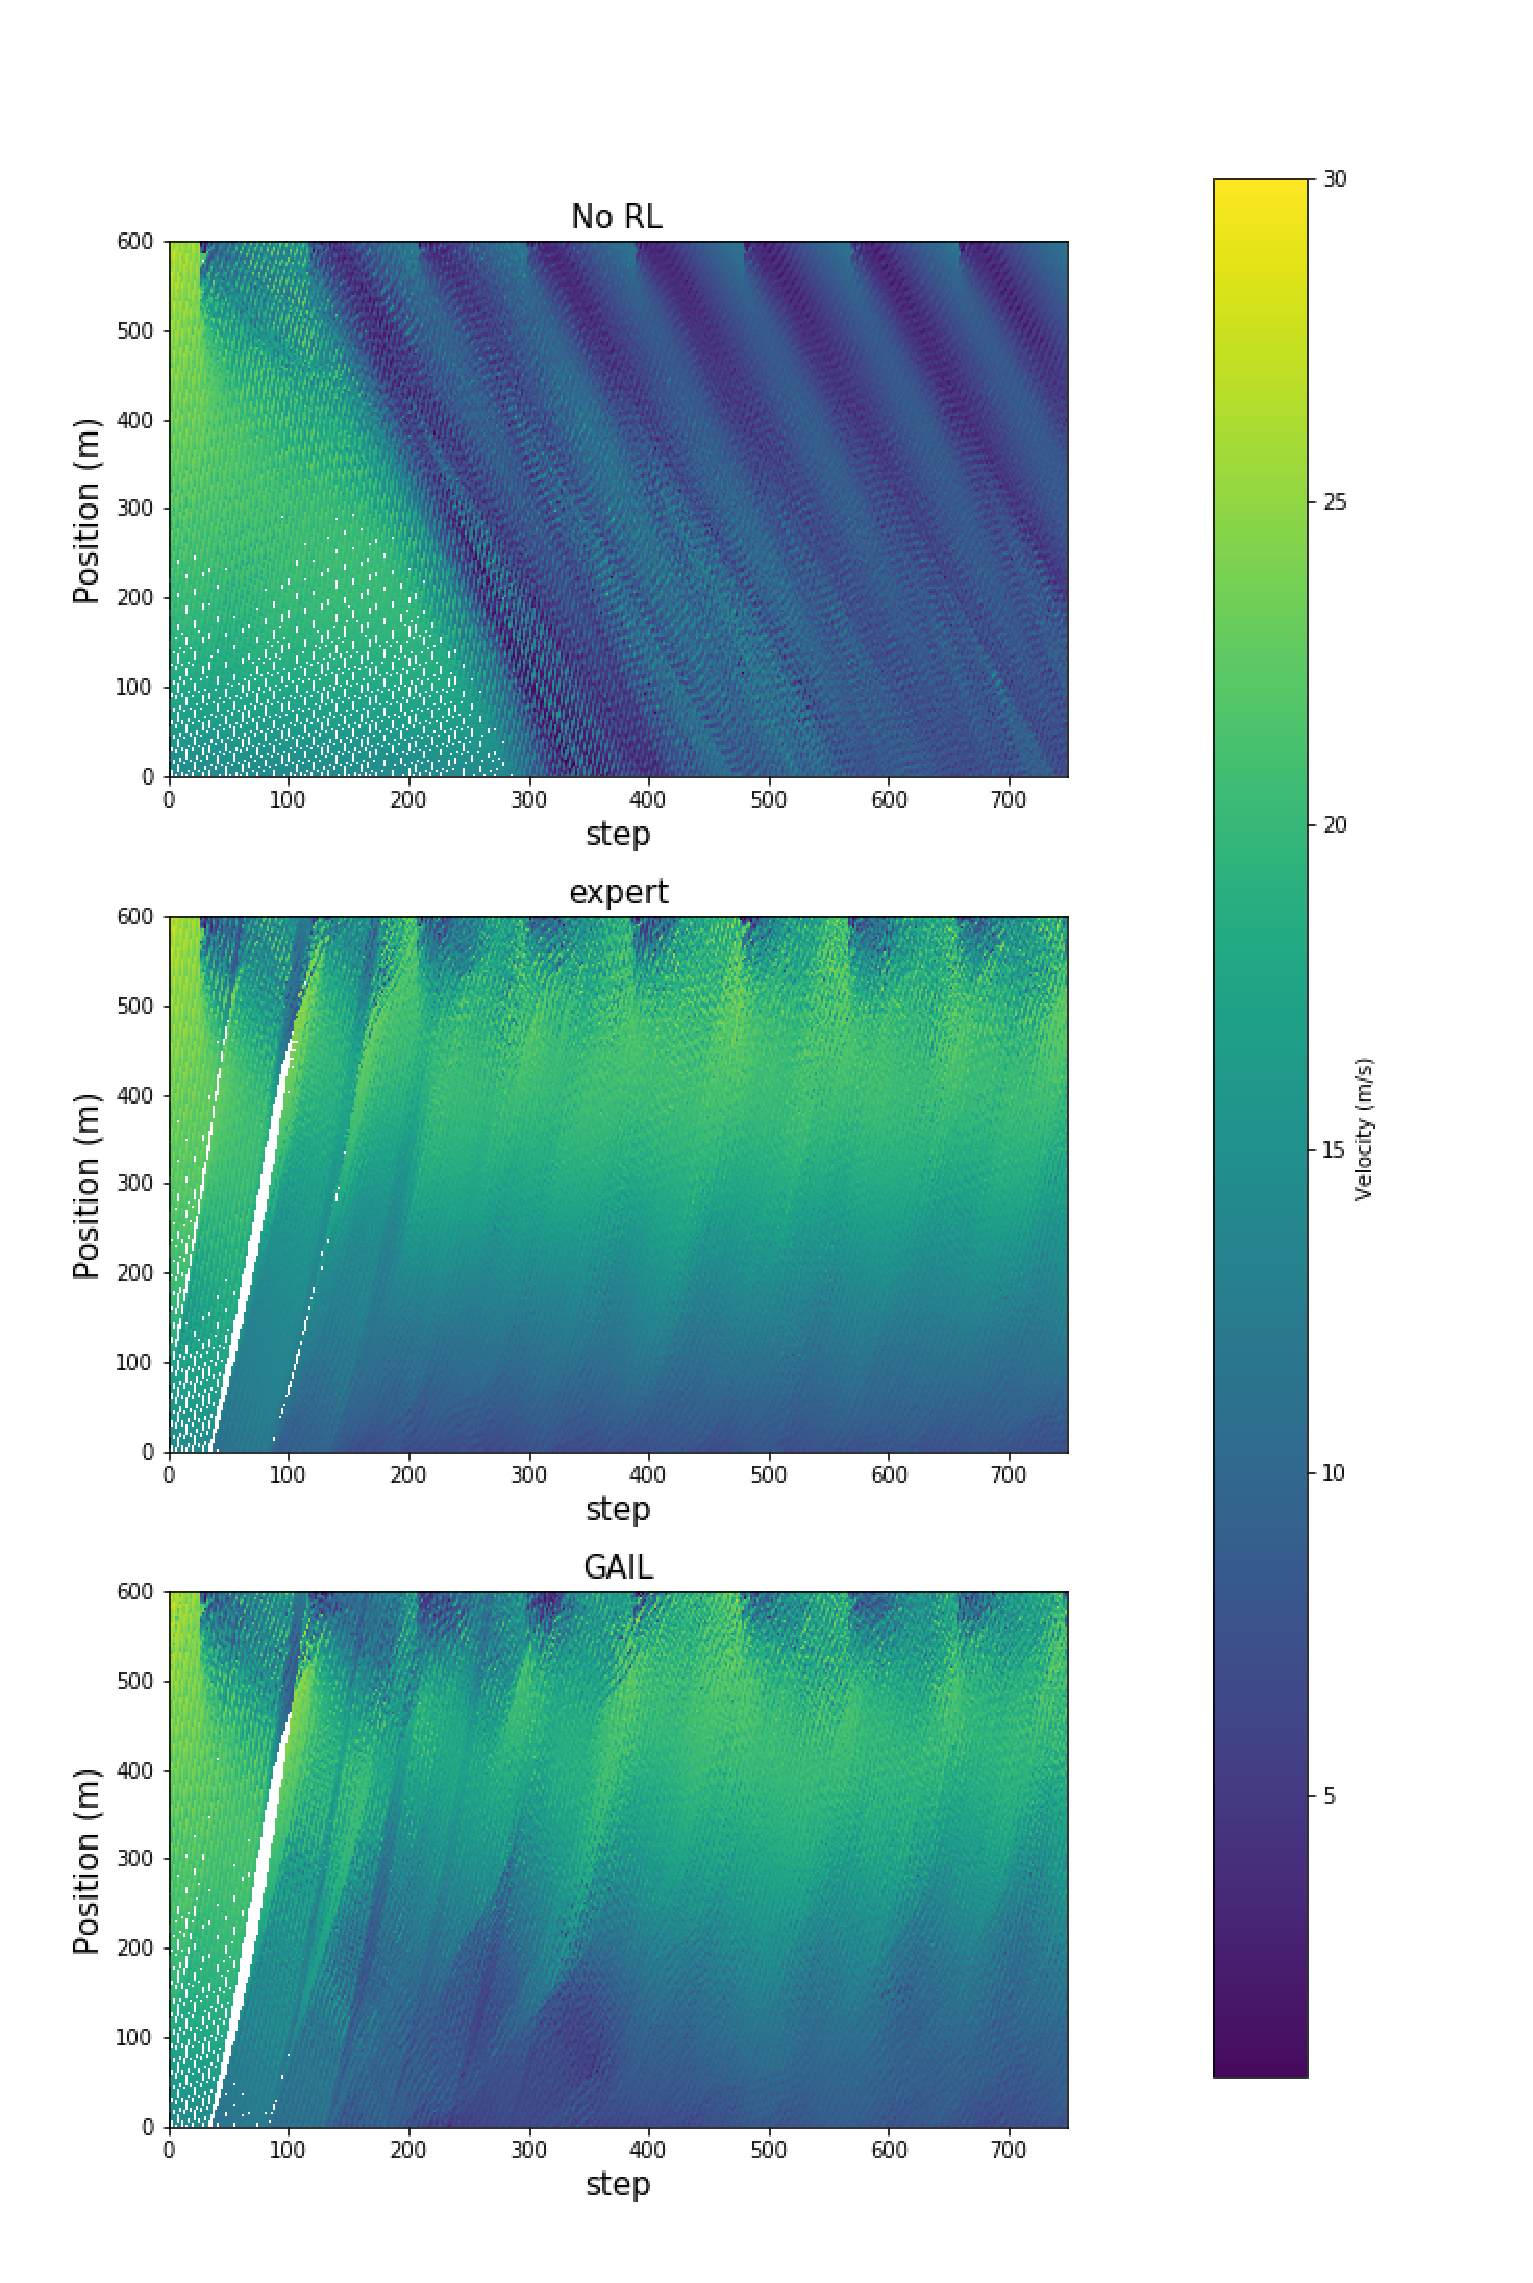
\includegraphics[width=10cm]{img/congestion.eps}
    \caption{Heat map of congestion level on the road. The results are averaged by 50 episodes. From top, the figures are the results of "No RL", "PPO" and "GAIL". If there are slow cars on the road, it appears as blue part. The "No RL" result has stop-and-go waves as blue lines propagating from top left to bottom right, but the other results doesn't have that.}
    \label{fig:congestion}
    \end{center}
\end{figure}

\begin{figure}[]
    \begin{center}
    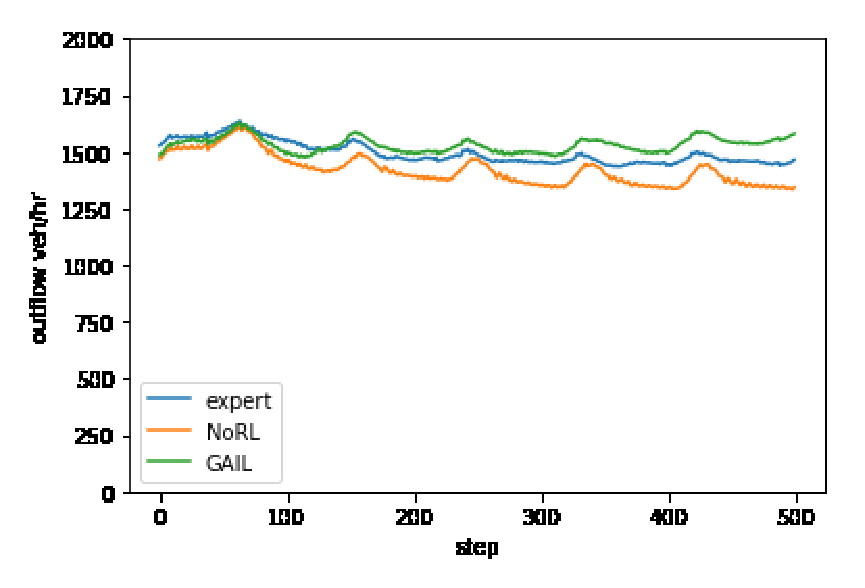
\includegraphics[width=9cm]{img/outflow.eps}
    \caption{Outflow rate during one episode. The results are averaged by 50 episodes. These three results keep almost the same outflow rate, around 1500 veh/hr.}
    \label{fig:outflow}
    \end{center}
\end{figure}

\begin{figure}[]
    \begin{center}
    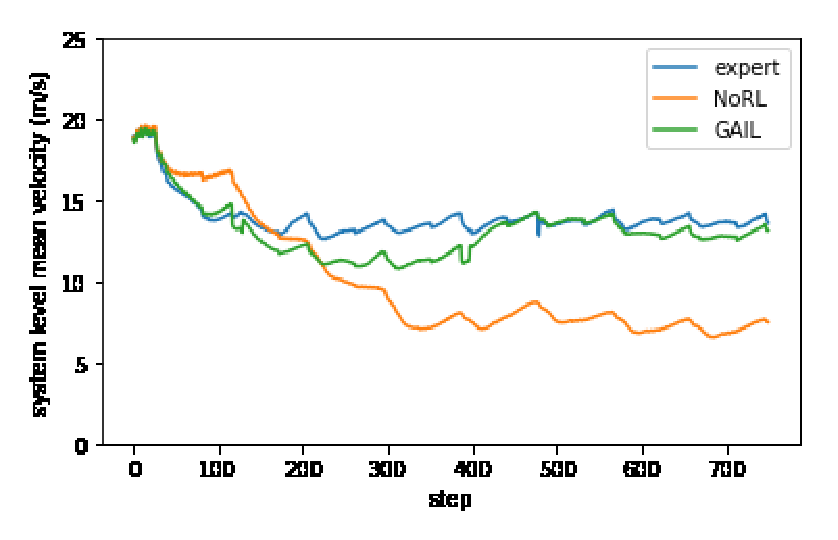
\includegraphics[width=9cm]{img/velocity.eps}
    \caption{Mean velocity of the traffic. The results are averaged by 50 episodes. Compared to the result of "No RL", GAIL and PPO keep high velocity during the episode.}
    \label{fig:velocity}
    \end{center}
\end{figure}

\section{Discussion}\label{sec:discussion}

This research solves the problems of the previous work\cite{Kreidieh2018}. The two problems of the previous work is, the limitation of the number of the RL cars and the vulnerability of the master node. Compared to \cite{Kreidieh2018}, multi-agent doesn't require one master node to control all the vehicles, and each RL cars works independently. Therefore, the multi-agent one is safer than the one master node and more flexible. However, there are still many space to improve. The future works are as follows.

\subsection{Model generalization}
The agent is trained only on the merge network, so it is not guaranteed that it works on the other environments(e.g. figure eight, grid, bottleneck (see Fig. \ref{fig:envs})). A future work is to train a more general agent which works in a variety of environments. As for the environments, there might be some problems on the original flow benchmarks. As mentioned in \ref{sec:experiments}, agents can lean how to reduce the outflow rate in the merge network. If the agent stop at the start point on the real traffic, congestion can happen at the start point. To measure the performance of the agent more accurately, better benchmark which prevents this phenomenon is necessary.

\subsection{For the real world application}
The results of the GAIL shows the potential to reproduce an expert performance from trajectories. IL can solve the reward function problem, and it is useful especially in the real world tasks. In the real world, it is easy to obtain the trajectories using some sensors. The obtained trajectories can be used as an expert, and from which it is possible to reconstruct an agent imitating the behavior. The problem of GAIL is its sample inefficiency. GAIL consumes about 1 million samples to train an agent, and it requires 20 CPUs and 150 iteration of simulation. To find more sample efficient algorithms is a future work.

\subsection{Better algorithms}
Another problem of GAIL for this task is the biased trajectory from the expert. The expert agent keeps a certain length of bumper-to-bumper distance and accelerates when there is a enough distance. After a few seconds from time $t=0$, all the RL cars have enough distance and they converge to a stable traffic where they can drive with constant speed(free-flow). The problem is that the most of the part of the expert trajectory is from the free-flow traffic. Therefore, the number of samples from congested traffic is less than that of the free-flow traffic, so the expert sample is biased. It might make the training slower. DQN\cite{Mnih2013} has a similar problem, but it is solved by prioritized experience replay\cite{Schaul2015}. The idea is to use the sample which have huge effects on the training. This idea can be used in the IL work and solve the problem. To apply such less biased algorithm to the traffic control is another future work.

One solution for sample efficient algorithm is model-based RL. \cite{Nagabandi2017}, \cite{Nagabandi} apply Model Predictive Control(MPC) to the RL training part, and successfully reduce the number of samples to train an agent controlling the real world robot. Although the model-predictive control is powerful as a model-based method, some changes are required if we want to apply it for the mixed-autonomy task. The problem is due to the fact that the reward function\ref{eq:newR} cannot be calculated from the state space, since it contains the mean velocity of the all the cars. Most of the model-based RL predicts the next state $s_{t+1}$ from the current state $s_t$ and action $a_t$ pair, and calculate the reward $r_{t+1}$ from the pair. Some predictions of the reward function or the other approach are necessary since the $r_{t+1}$ cannot be calculated from the pair in this task. 

A promising approach is using inverse RL\cite{Ng2000}. Inverse RL reconstructs the reward function from the trajectory of a policy. Since the generated reward function by inverse RL is estimated from the state and action pair, it is possible to use the reward to the MPC. In short, the algorithm proposal consists of two steps, 1. reconstruct the reward function $r_t(s_t, a_t)$ from an expert, 2. use MPC and do model-based RL to train the agent.

\bibliographystyle{unsrt}
\bibliography{mybib} 
%----------------------------------------------------------------------------------------


\end{document}